\section[DoS Extension]{How to Use the DoS Extension of the WS-Attacker}
\label{sec:how_to_use_dos_extension}

This guide shows how to use the DoS attack plugins of the WS-Attacker.
The DoS attack plugins are based on the paper \emph{A New Approach towards DoS Penetration Testing on Web Services} presented on ICWS 2013~\cite{wsattackerDoS}.

\subsection{General Design of the WS-Attacker DoS Extension}
\label{sec:design_DoS_extension}

The design of the automated Web service DoS attack tool is shown in Figure~\ref{fig:architectureDosAttackTool} using a UML-based activity diagram to describe the high level program flow.
This newly created design is especially tailored towards solving the problems caused by using the blackbox approach when measuring the attack success.\newline

For each Web service specific DoS attack, the following nine parameters have to be set up:
\begin{itemize}
  \item M = number of sequential (un)tampered requests per thread 
  \item N = number of parallel threads 
  \item T = milliseconds between continuous untampered testprobe requests
  \item K = milliseconds between each (un)tampered request 
  \item X = seconds between receiving last untampered request and sending first untampered request 
  \item S = seconds between receiving last tampered request and finalization (end) of the attack 
  \item L = number of network stability test requests
  \item R = milliseconds between each network stability test request 
  \item Message = the string will be used to create a tampered request.\\
  By default, this variable holds the original SOAP request of the targeted Web service.\\
  The string value can be set to an arbitrary value. No valid XML is required.\\
  If set by the attack developer, the string can hold a payload placeholder. This allows a tester to place the payload to the position required for the attack to work.
\end{itemize}

\newpage
Furthermore, the following two boolean values have to be set: 
\begin{itemize}
  \item Boolean attackStop\\If true, the attack will finalize automatically after S seconds. Otherwise, the attack will run until the user finalizes the attack manually. 
  \item Boolean performNetworkStabilityTest\\If true, network stability test will get performed. Otherwise, it will get skipped.
\end{itemize}

The program flow when executing a single attack is shown in Figure~\ref{fig:architectureDosAttackTool}.
\begin{landscape}
  \begin{figure}[!ht]
	  \centering
	  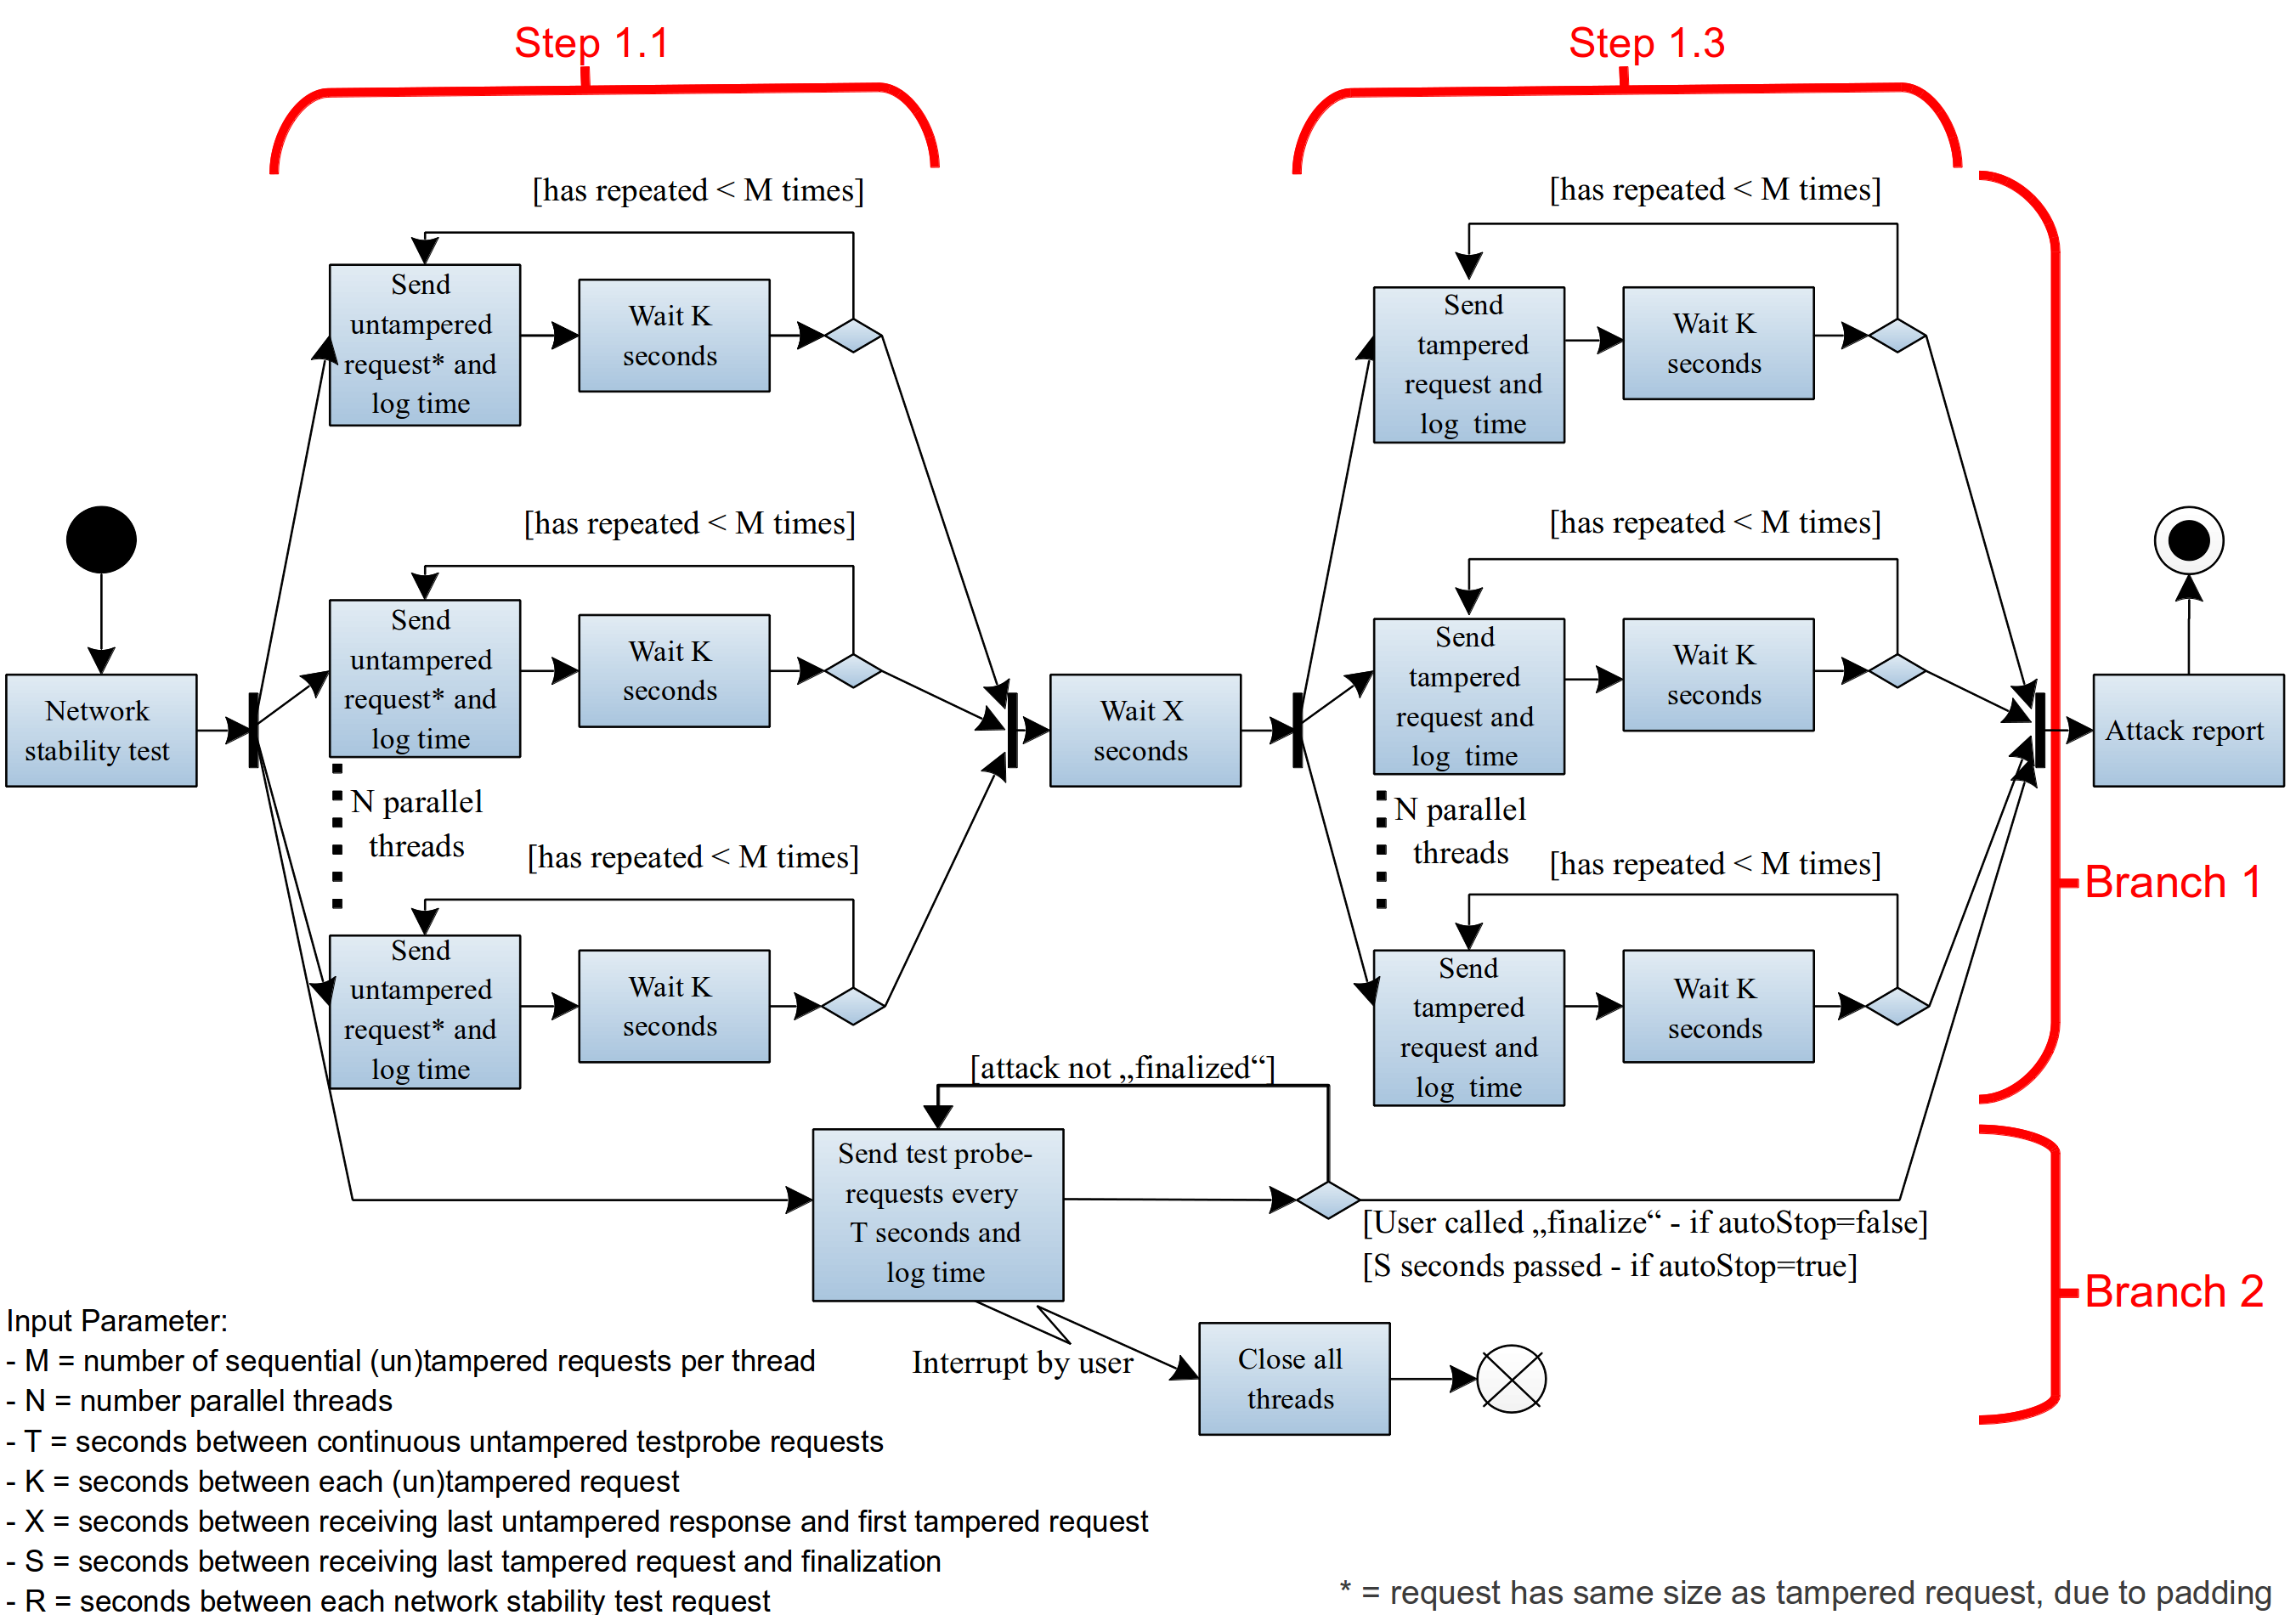
\includegraphics[width=21cm]{img/architecture.png}
	  \caption{Architecture of an automated Web service specific DoS attack tool}
	  \label{fig:architectureDosAttackTool}
  \end{figure}
\end{landscape}

The steps in Figure~\ref{fig:architectureDosAttackTool} are as follows:
  \begin{enumerate}
    \item Test network stability\par When the program is started, a network stability test will get performed (only when enabled by the user). The outcome will tell the tester whether or not a penetration test is feasible under the given network delays. The result has just informative character. A negative result of the network stability test will not stop the program. 
    \item Perform attack\par After the network stability test, the program flow splits into two branches.  
    \begin{enumerate}
      \item Branch 1: Perform attack including error correction\par This branch performs the actual attack. However, errors might occur. Therefore, branch 1 is split into three substeps.
      \begin{enumerate}
	\item Branch 1 - step 1:\\Open N threads in parallel and send M untampered requests per thread.\par Each thread induces a delay of K seconds between each request. The delay timer starts as soon as the the client tries to send the request. It is not waited until a response is returned. Otherwise, reproducible results would not be possible.
	\item Branch 1 - step 2:\\Wait for X seconds. 
	\item Branch 1 - step 3:\\Open N threads in parallel and send M tampered requests per thread.\par Each thread induces a delay of K seconds between each request.
      \end{enumerate}  
      \item Branch 2: Simulate regular user who uses the Web service while attack is running\par Branch 2 continuously sends untampered requests to the Web service with a delay of T seconds between each request. This process continues until the attack is finalized.  The attack finalization can be triggered by the user if the boolean attackStop is set to false. Otherwise, the attack will stop automatically after S seconds.
    \end{enumerate}
    \item Attack results\par Branch 1 and branch 2 are finished. All logged data is grouped and analyzed by the program. Each logged request will get assigned to an discrete interval. By default the interval length is one second. 
    The attack results will be presented in the attack report. Options for saving the results are also presented.
  \end{enumerate}


This software design was newly created; incorporating the goal of creating a fully automated Web service specific DoS attack tool using the blackbox approach. 
The design meets the following requirements:

\minisec{Automated Crafting and Sending of Attack Messages for Chosen DoS Attack}
\label{sec:ImpAutomatedSending}
All requests are created by the DoS attack tool.
Based on the chosen attack parameters, the requests get sent automatically for the defined number of times. 

\minisec{Fitness for Various Load Scenarios}
\label{sec:ImpLoadScenario}
By setting up the parameters 
\begin{enumerate}
  \item M = number of sequential (un)tampered requests per thread 
  \item N = number parallel threads 
  \item K = milliseconds between each (un)tampered request
\end{enumerate}
the penetration tester is able to define arbitrary load scenarios. 

\minisec{Fitness for Various Test Scenarios}
\label{sec:ImpTestScenarios}
The design shown in Figure \ref{fig:architectureDosAttackTool} allows for testing of two distinct test scenarios. 
\begin{enumerate}
  \item Test for vulnerability.\\
  A vulnerability test can be conducted by running an attack with very few requests.
  Ideally, one thread with one request is enough to decide whether or not the target is vulnerable to the chosen Dos attack.
  
  \item Test for attack effect on third party users.\\
  A test that checks if third party users are affected can be achieved by increasing the duration of the attack and the load per interval. 
  There is no default option provided for this test scenario. The hardware performance of the tested system can vary heavily. 
  Therefore, a tester has to manually vary the parameters and rerun the test until the desired result is achieved on a vulnerable system.\\
\end{enumerate}

\minisec{Elimination of Errors}
\label{sec:ImpErrors}
Elimination of the errors takes place in branch 1 of the activity diagram. 
Step 1.1 and step 1.3 both cause the same load on the network:
\begin{itemize}
 \item The time pattern in which the messages are sent is equal.
 \item The message size of untampered and tampered requests is equal, due to message padding.
\end{itemize}
The only difference between these steps is that step 1.1 sends untampered requests and step 1.3 sends tampered requests.  
When using this pattern, any significant difference in roundtrip time between tampered and untampered requests must be caused by the attack payload.\\

\minisec{Exclusion of Subattacks}
Some attacks are composed of different subattacks. However, a tester might want to test for only one of the subattacks. 
In this case, the tampered request has to hold the payload of the entire attack. The untampered request has to hold the payload of the subattacks the tester doesn’t want to test for. 
When calculating the attack success metric, only the impact of the subattack that is not included in the untampered request is considered.



\subsection{Walktrough example of a coercive Parsing Attack}
\label{sec:walkthrough_example}

In the following a full attack walkthrough of a coercive parsing DoS vulnerability test is given. Information on the coercive parsing attack can be found here: \url{http://ws-attacks.org/index.php/Coercive_Parsing}
The general steps required to perform a DoS vulnerability test are as follows: 
\begin{enumerate}
    \item Load the WSDL.
    \item Submit a test request.
    \item Select and configure the ``coercive parsing'' attack plugin.
    \item Start the attack.
    \item View attack results.
\end{enumerate}

The steps needed to run any other DoS attack plugin are similar. 
Only in step 3 slight differences can occur, since the attack specific parameters might vary based on the chosen attack.


\subsubsection{Load the WSDL}
\label{sec:loading_a_wsdl_dos}

After starting WS-Attacker, the GUI appears and offers an input field to enter the location
of the WSDL, see Figure \ref{fig:dosStep1}.

\begin{figure}[h!]
    \begin{center}
        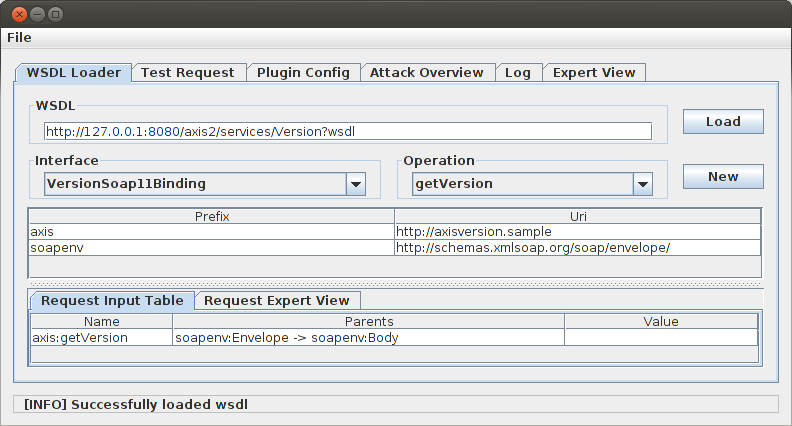
\includegraphics[width=0.8\textwidth]{img/dosStep1}
    \end{center}
    \caption{Loading the WSDL.}
    \label{fig:dosStep1}
\end{figure}

In this testcase the WSDL file \url{http://127.0.0.1:8080/axis2/services/Version?wsdl} is loaded. All other parameters are left at their default values. 
For more information on the other parameters please refer to the general WS-Attacker documentation.

\subsubsection{Submit a test request}
\label{sec:submitting_a_test_request_dos}
Next step is to do a test request: Figure \ref{fig:dosStep2} shows
the test request and the corresponding response. 
The test request is very important. It is used as the baseline request for all further testing. 
Based on this test request, all attack payloads will be build later on.

\begin{figure}[h!]
    \begin{center}
        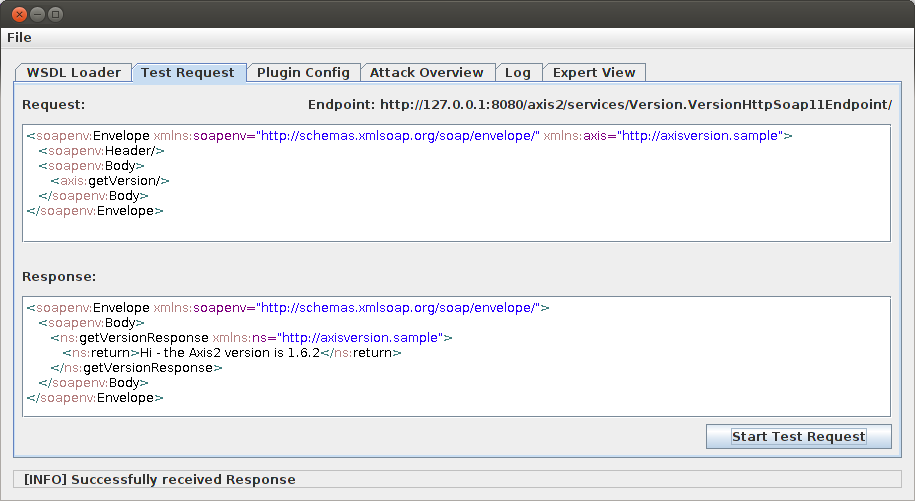
\includegraphics[width=0.8\textwidth]{img//dosStep2}
    \end{center}
    \caption{Submitting a test request.}
    \label{fig:dosStep2}
\end{figure}

\subsubsection{Select and configure the attack plugins}
\label{sec:attack_plugin_configuration_dos}

Next the attack plugin is selected and configured. In this scenario, only the coercive parsing DoS attack
is chosen. As soon as the plugin is selected, the attack options will show up on the right side (Figure \ref{fig:dosStep3}). 

\begin{figure}[H]
    \begin{center}
        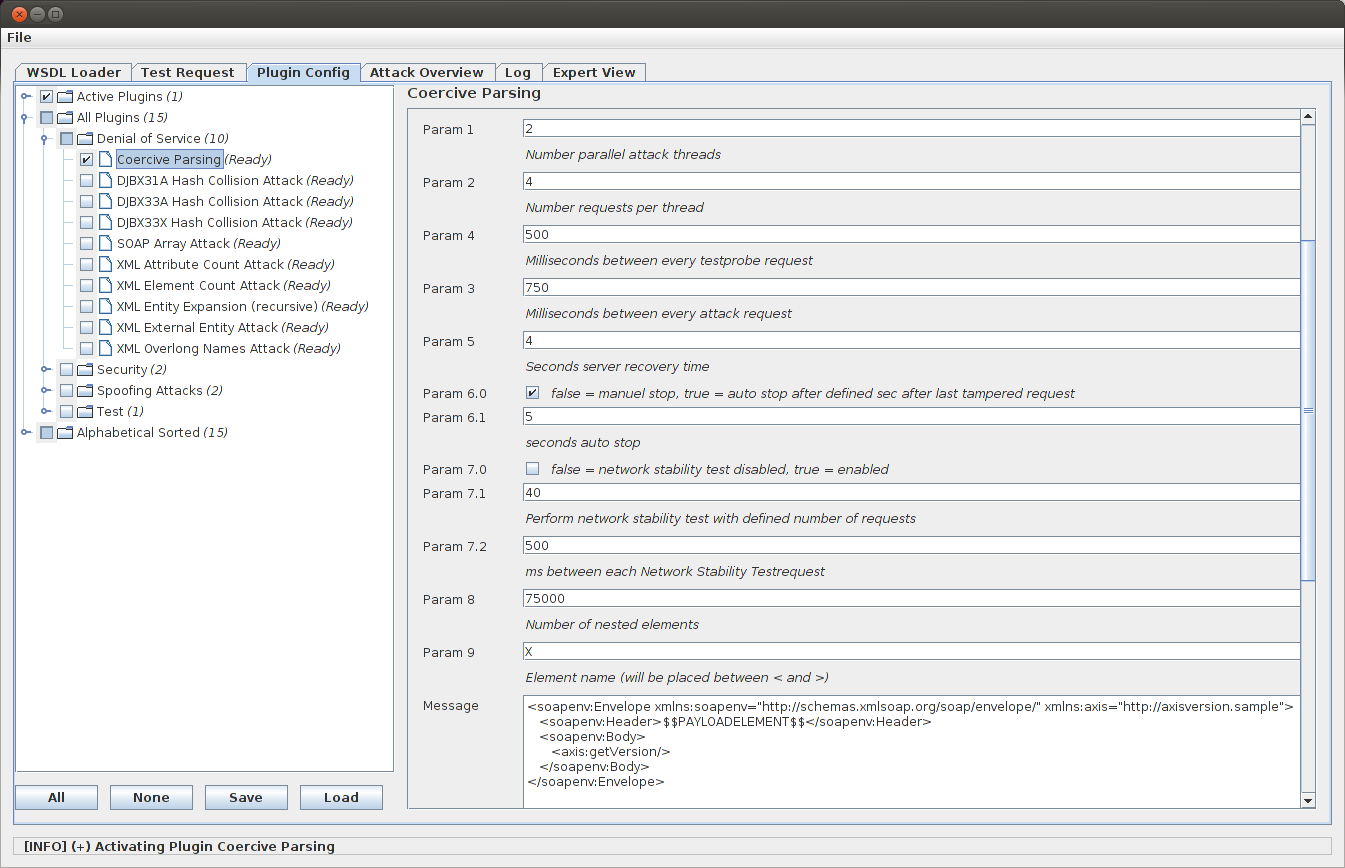
\includegraphics[width=0.95\textwidth]{img/dosStep3_1.png}
    \end{center}
    \caption{Selected attack plugin ``coercive parsing''}
    \label{fig:dosStep3}
\end{figure}

In general the DoS attack plugin can be left at its default parameters. 
Any vulnerable Web Service should be clearly marked as vulnerbale with the default parameters. 

The plugin offers the following attack specific options:
\begin{itemize}
    \item Number of nested elements \\The default number is at 75000. This means 75000 XML elments will be nested within each other.
    \item Element name (will be placed between < and >) \\The default element name is ''x``.
\end{itemize}

The following DoS attack extension specific parameters can be left unchanged:
\begin{itemize}
    \item Number parallel attack threads
    \item Number requests per thread 
    \item Milliseconds between every testprobe request
    \item Milliseconds between every attack request
    \item Seconds server recovery time
    \item Auto stop switch
    \item seconds auto stop
    \item Network stability test 
    \item Perform network stability test with defined number of requests
    \item Ms between each Network Stability Testrequest
    \item Message
\end{itemize}

\subsubsection{Start the attack}
\label{sec:starting_the_attacks_dos}

The last step is to start the attack. 
Just switch to the \"Attack Overview\"-tab and press the start button. See Figure~\ref{fig:dosStep4}.

\begin{figure}[H]
    \begin{center}
        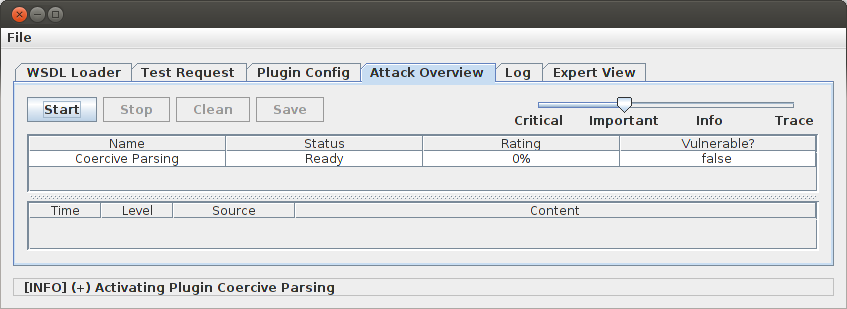
\includegraphics[width=0.95\textwidth]{img/dosStep4.png}
    \end{center}
    \caption{Starting the attack.}
    \label{fig:dosStep4}
\end{figure}

While the attack is running
\begin{figure}[H]
    \begin{center}
        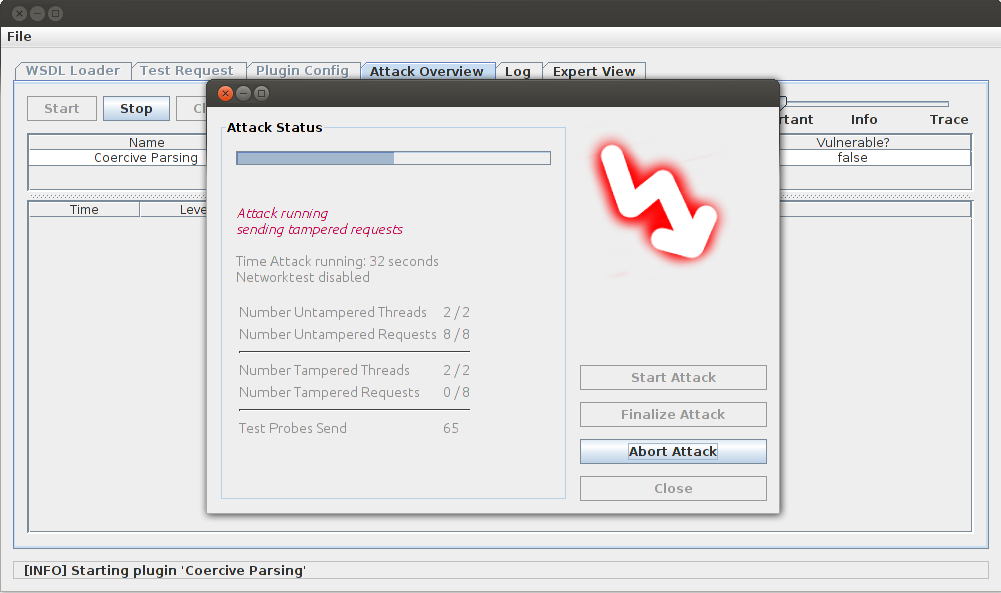
\includegraphics[width=0.8\textwidth]{img/dosStep4_1.png}
    \end{center}
    \caption{Attack is running}
    \label{fig:dosStep4_1}
\end{figure}


\subsubsection{View attack results}
\label{sec:view_results}

Once the attack is finished, the status column should turn green. The column ''Rating`` and ''vulnerable`` already give a rough hint of the attack success.
As shown in Figure~\ref{fig:dosStep4_2}, the tested Web Service is rated as 100\% vulnerbale. 
\begin{figure}[ht!]
    \begin{center}
        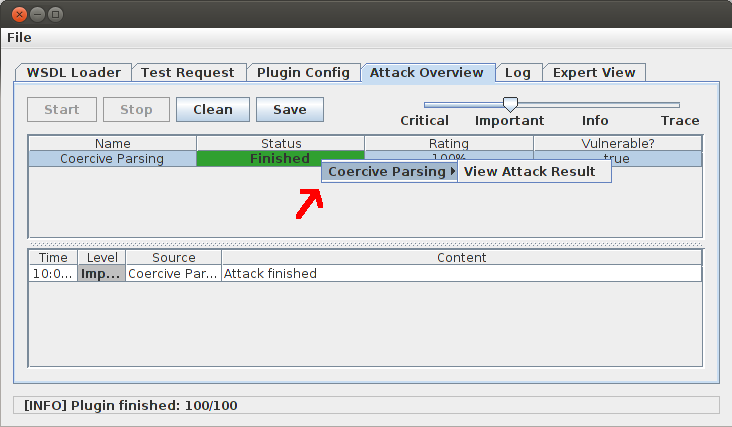
\includegraphics[width=0.95\textwidth]{img/dosStep4_2.png}
    \end{center}
    \caption{Penetration test finished}
    \label{fig:dosStep4_2}
\end{figure}

In Order to see a detailed attack description, just right click the coercive parsing attack row. 
A sub menu will show that lets you choose the ''View Attack Results`` option. The final attack result are presented in Figure~\ref{fig:dosStep4_3}.
\begin{figure}[H]
    \begin{center}
        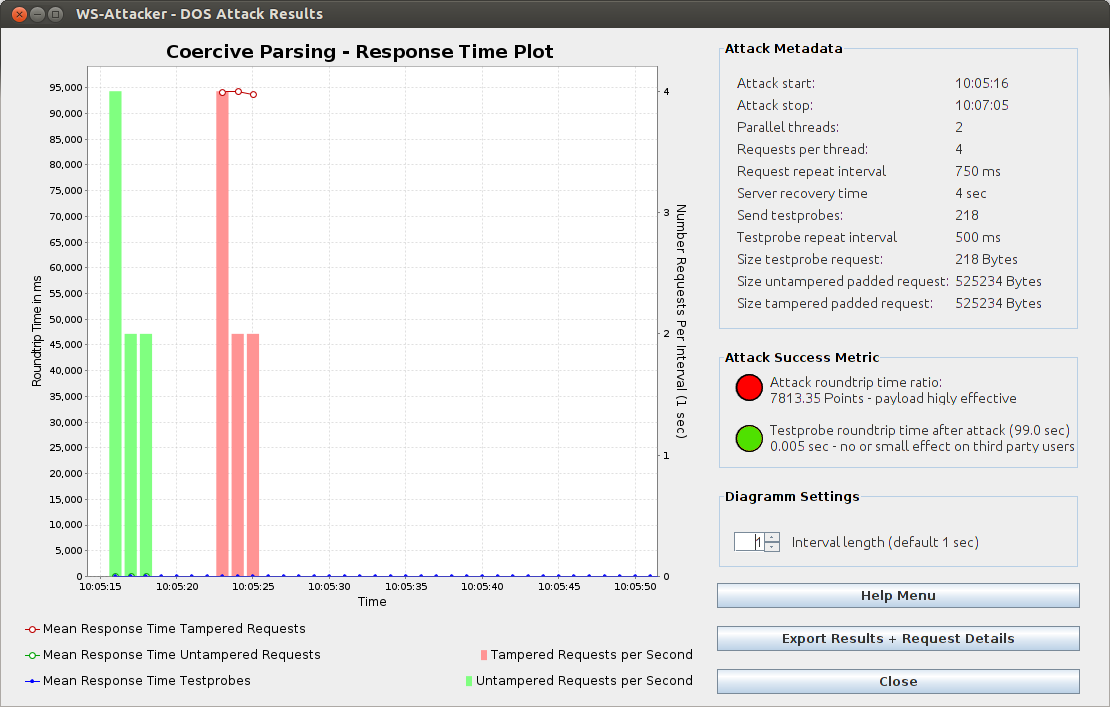
\includegraphics[width=0.95\textwidth]{img/dosStep4_3.png}
    \end{center}
    \caption{View attack result details}
    \label{fig:dosStep4_3}
\end{figure}
As shown in Figure~\ref{fig:dosStep4_3}, the tested Web Service is clearly vulnerable. 
The ''attack roundtrip time ratio`` is at 7813. This means that on average, the response time of a tampered request is 7813 times longer than a regular untampered request under the same load scenario.

The attack results with all details (including all payload requests) can be saved as Txt-File and Jpg-File by clicking the button ''Export Results + Request Details``.
A new instance of Firefox should pop up that provides links to the result files.
